\documentclass[12pt,a4paper]{report}
\usepackage[utf8]{inputenc}
\usepackage[T1]{fontenc}
\usepackage[french]{babel}
\usepackage[top=1.8cm, bottom=1.8cm, left=1.8cm, right=1.8cm]{geometry}
\usepackage[linktocpage,colorlinks=false]{hyperref}
\usepackage{graphicx}
\usepackage{epsfig}
\usepackage{amssymb}
\usepackage{amsmath}
\usepackage{array}
\usepackage{subfig}
\usepackage{multicol}
\usepackage{caption}
\usepackage{algorithm}
\usepackage{color}
\usepackage{algorithmic}
\usepackage{listings}
\usepackage{url}
\usepackage{fullpage}
\usepackage{color}
\usepackage[table]{xcolor}
\usepackage{listings}

\definecolor{darkWhite}{rgb}{0.94,0.94,0.94}

\hypersetup{
    colorlinks=true,
    breaklinks=true,
    urlcolor=black,
}
\parskip=5pt
\begin{document}
\begin{titlepage}
\newgeometry{top=0.5in,right=0.5in,left=0.5in,bottom=1in}	


 \begin{center}
	\textbf{\centering  Université de Paris Saclay } 

\end{center}

	
	

\begin{figure}[h]
    \centering
    
\includegraphics[width=5cm]{images/UVSQlogo.png}
\end{figure}
	\vspace{2cm}

\begin{center}
	\Huge{\textbf{Calcul Sécurisé}	}
\end{center}

\vspace{2cm}
\hrule	
\begin{center}
\Huge{\textbf{ Attaque par faute sur DES }	}
\end{center}
\hrule
\vspace{1cm}
\begin{center}
	\Large{\textbf{Par :} }
	
\end{center}

\begin{center}
\large{\textbf{Imad BOUKEDJANI 22305124}}
\end{center}

\vspace{1cm}

\hrule

\begin{center}
\large{\textbf{Lien Github : } } 
\end{center}
\vspace{1cm}

\begin{center} 
\large{\textbf{\href{https://github.com/lmaaaad/Attack-par-fautes-sur-DES}{https://github.com/lmaaaad/Attack-par-fautes-sur-DES} }}
\end{center}
\hrule

\end{titlepage}

\newpage
\renewcommand{\thesection}{\arabic{section}}

\tableofcontents
\newpage
\section{Attaque par faute sur le DES}

Une attaque par faute implique de modifier le résultat d'un sous-calcul pour obtenir une information secrète. Ainsi, cette modification entraînera intentionnellement une erreur.
Cette attaque est physique, car elle nécessite une intervention directe sur les composants électroniques pour altérer certaines bits. Dans le contexte du DES, une attaque par faute sur la valeur de sortie $R_{15}$ du $15^{e}$ tour implique que l'attaquant altère volontairement la valeur de $R_{15}$ . 

\begin{center}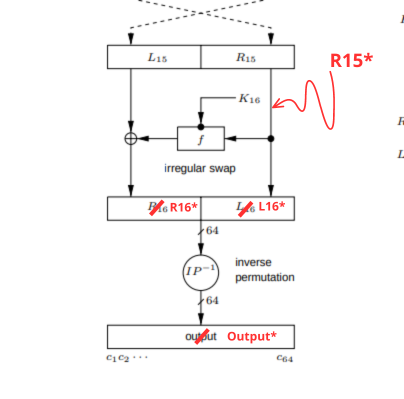
\includegraphics[scale=1]{images/DES.png}
\end{center}

À partir de cette attaque, la clé secrète utilisée par la victime peut être retrouvée à partir de la sous-clé $K_{15}$. On suppose ici que nous sommes l'attaquant et que nous avons réussi à obtenir de la victime le message clair associé à son message chiffré (avec une clé inconnue pour le moment, qui est à trouver).  En outre, la victime a fourni 32 chiffres (toujours avec la même clé) et nous avons réussi à attaquer par erreur. Donc, afin de mener à bien cette attaque de manière adéquate, il est nécessaire de trouver $K_{16}$ et en déduire $K$. La description de cette attaque sera présentée plus loin.  

\newpage

\section{Application concrète}

\subsection{Question 1}

Cette attaque par faute sur le dernier tour du DES comporte plusieurs étapes : 

\begin{itemize}
	\item Étape 1 : Trouver $R_{15}$ à partir du chiffré juste et les $R_{15}*$ à partir des chiffrés faux. \newline Pour cela, on fait une permutation initiale (qui annule la permutation finale $IP^{-1}$) pour trouver $L_{16}$ et $R_{16}$. On fera de même pour $R_{15}*$ à partir des chiffrés faux. On peut désormais écrire les formules suivantes : \newline \newline $R_{16}= L_{15} \oplus f(K_{16}, R_{15})$ et $L_{16}=R_{15}$ pour le chiffré juste. 
	\newline $R_{16}*= L_{15} \oplus f(K_{16}, R_{15}*)$ et $L_{16}*=R_{15}*$ pour les chiffrés faux. \newline \newline Le but ici est d'obtenir $K_{16}$ : pour cela, on fait le XOR entre $R_{16}$ et un $R_{16}*$. Ce qui nous donne l'équation suivante : \newline \newline
	$R_{16} \oplus R_{16}* =  L_{15} \oplus f(K_{16}, R_{15}) \oplus L_{15} \oplus f(K_{16}, R_{15}*)$ \newline 
	%\newline \Leftrightarrow g$
	Les $L_{15}$ s'annulent et on obtient : $R_{16} \oplus R_{16}* = f(K_{16}, R_{15}) \oplus f(K_{16}, R_{15}*)$ \newline \newline
	Or, $f(K_{i+1}, R_{i})=P(S(E(R_{i})\oplus K_{i+1})) = P(S_1(E(R_i)\oplus K_{i+1})_{b_1\to b_6} || ... || S_8(E(R_i)\oplus K_{i+1})_{b_{43}\to b_{48}})$ \newline
		
	\item Étape 2 : Pour chaque chiffré faux (associé à son $R_{15}*$), établir 8 équations pour chaque boîte-S. 

\[
\begin{cases}
    P^{-1}(R_{16}\oplus R_{16}*)_{b_1\to b_4} &= S_1(E(R_{15})\oplus K_{16})_{b_1\to b_4} \oplus S_1(E(R_{15}*)\oplus K_{16})_{b_1\to b_4} \\
    P^{-1}(R_{16}\oplus R_{16}*)_{b_5\to b_{8}} &= S_2(E(R_{15})\oplus K_{16})_{b_5\to b_{8}} \oplus S_2(E(R_{15}*)\oplus K_{16})_{b_5\to b_{8}} \\
    P^{-1}(R_{16}\oplus R_{16}*)_{b_{9}\to b_{12}} &= S_3(E(R_{15})\oplus K_{16})_{b_{9}\to b_{12}} \oplus S_3(E(R_{15}*)\oplus K_{16})_{b_{9}\to b_{12}} \\
    P^{-1}(R_{16}\oplus R_{16}*)_{b_{13}\to b_{16}} &= S_4(E(R_{15})\oplus K_{16})_{b_{13}\to b_{16}} \oplus S_4(E(R_{15}*)\oplus K_{16})_{b_{13}\to b_{16}} \\
    P^{-1}(R_{16}\oplus R_{16}*)_{b_{17}\to b_{20}} &= S_5(E(R_{15})\oplus K_{16})_{b_{17}\to b_{20}} \oplus S_5(E(R_{15}*)\oplus K_{16})_{b_{17}\to b_{20}} \\
    P^{-1}(R_{16}\oplus R_{16}*)_{b_{21}\to b_{24}} &= S_6(E(R_{15})\oplus K_{16})_{b_{21}\to b_{24}} \oplus S_6(E(R_{15}*)\oplus K_{16})_{b_{21}\to b_{24}} \\
    P^{-1}(R_{16}\oplus R_{16}*)_{b_{25}\to b_{28}} &= S_7(E(R_{15})\oplus K_{16})_{b_{25}\to b_{28}} \oplus S_7(E(R_{15}*)\oplus K_{16})_{b_{25}\to b_{28}} \\
    P^{-1}(R_{16}\oplus R_{16}*)_{b_{29}\to b_{32}} &= S_8(E(R_{15})\oplus K_{16})_{b_{29}\to b_{32}} \oplus S_8(E(R_{15}*)\oplus K_{16})_{b_{29}\to b_{32}}\newline
    
\end{cases}
\]

	
	 \item Étape 3 : Éliminer les équations dont $P^{-1}(R_{16}\oplus R_{16}*)_{b_x\to b_y}$ vaut $0$ puisqu'elles n'apporteront aucune information sur la portion de sous clé $K_{16}$. \newline
	
	\item Étape 4 : Faire une attaque exhaustive(Brute-Force) sur la sortie de chaque boîte-S  $S_z(E(R_{15})\oplus K_{16})_{b_{x}\to b_{y}}$ , pour chaque élément, on déduit les possibles valeurs d'entrée de la boîte-S $E(R_{15})\oplus K_{16}$. Ainsi, on en déduit une possible $K_{16}$. \newline
	
	\item Étape 5 : Pour chaque $K_{16}$ possible, calculer $S_z(E(R_{15}*)\oplus K_{16})_{b_{x}\to b_{y}}$ et regarder si $P^{-1}(R_{16}\oplus R_{16}*)_{b_{x}\to b_{y}} = S_z(E(R_{15})\oplus K_{16})_{b_{x}\to b_{y}} \oplus S_z(E(R_{15}*)\oplus K_{16})_{b_{x}\to b_{y}}$. \newline Si c'est le cas, alors $K_{16}$ en question devient une portion de clé candidate pour le chiffré faux associé. \newline 
	
	\item Étape 6 : Pour chaque boîte-S, il y a une liste de clés candidates pour chaque chiffré faux qui agit sur la portion de sous clé. Trouver pour chaque boîte-S l'intersertion des portions de clés candidates. Il y aura donc 1 portion de clé (sur 6 bits) par boîte-S. \newline
	
	\item Étape 7 : Concaténer les $8 \times 6$ bits pour obtenir la sous clé $K_{16}$. 
\end{itemize}


Dans notre cas, le message clair, le chiffré correct et les 32 chiffrés fautés nous sont déja fournis, ce qui équivaut a l'étape 1. On poursuit alors les opérations explicitées précédemment jusqu'a obtenir les ensembles d’ensembles de S-Box possibles au cours de l’étape 4.

\begin{enumerate}
    \item Boîte-S 1 : L’intersection des sous-ensembles vaut : $110011$
    \item Boîte-S 2 : L’intersection des sous-ensembles vaut : $111010$
    \item Boîte-S 3 : L’intersection des sous-ensembles vaut : $100010$
    \item Boîte-S 4 : L’intersection des sous-ensembles vaut : $111010$
    \item Boîte-S 5 : L’intersection des sous-ensembles vaut : $111011$
    \item Boîte-S 6 : L’intersection des sous-ensembles vaut : $110011$
    \item Boîte-S 7 : L’intersection des sous-ensembles vaut : $001001$
    \item Boîte-S 8 : L’intersection des sous-ensembles vaut : $110010$
    
\end{enumerate}

\subsection{Question 2}

On a donc en binaire : $110011111010100010111010111011110011001001110010$ \newline 

On obtient en hexadécimal pour $K_{16}$ :\color{red} \textbf{$K_{16} = CF$ $A8$ $BA$ $EF$ $32$ $72$} \color{black}

\begin{center}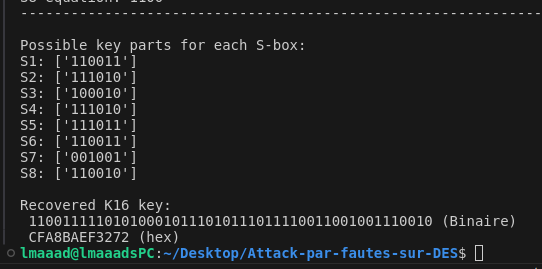
\includegraphics[scale=0.4]{images/resultat2}\end{center}

\section{Retrouver la clé complète du DES}

\subsection{Question 1}

Dans la question précédente, nous avons réussi à obtenir la clé secrète $K_{16}$ qui contient 48 bits. En analysant le schéma de création des 16 sous-clés (de 48 bits chacunes) à partir de la clé secrète (de 64 bits avec les 8 bits de parité), on peut en déduire la clé secrète a partir de : $K=PC^{-1}(PC^{-2}(K_{16}))$.

\begin{center}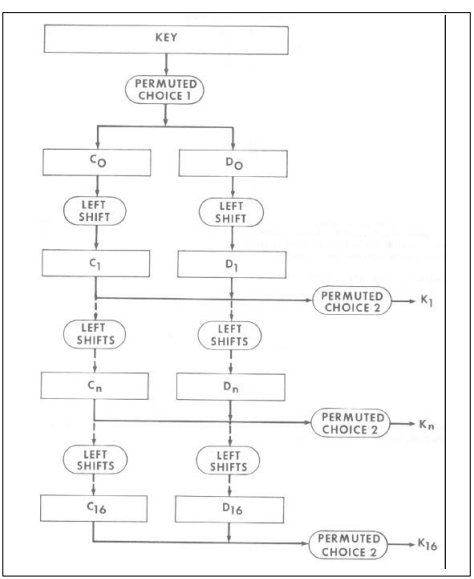
\includegraphics[scale=0.5]{images/key_CI-CD.png}\end{center}

\begin{itemize}
	\item Étape 1 : effectuer une permutation inverse $PC_{2}^{-1}(K_{16})$ afin d'obtenir $C_{16}$ et $D_{16}$.
	(C et D sont des registres sur $28$ bits ) Il est important de noter que lors de cette permutation inverse, 8 bits sont inconnus. En effet, on passe de $48$ bits à $2 \times 28 = 56$ bits. Il y a donc 8 bits qu'on ne peut déduire à partir de $K_{16}$. \newline
	
	\begin{center}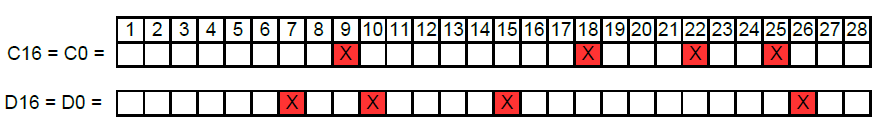
\includegraphics[scale=0.4]{images/C0_D0.png}\end{center}
	
 Et on sait que $C_{0}=C_{16}$ et $D_{0}=D_{16}$ puisque la somme des shifts circulaires donne $28$ qui correspond à la taille des blocs $C_i$ et $D_i$ , donc meme la taille des X ne changera pas  \newline
	

    	\item Étape 2 : Retrouver les 8 bits inconnus par une recherche exhaustive : $2^{8}=256$ cas possibles , dans une boucle on effectuer aussi une permutation inverse $PC_{1}^{-1}(C_{0}||D_{0})$ avec les cas possible afin d'obtenir la clé de 56 bits . apres cela, il nous reste les 8 bits de parité on nous assurant que chaque octet possède un nombre impair de bits à 1 . On on confirme les resultats avec une calculatrice en ligne (qui est fournie dans le sujet) jusqu'à ce que la clé nous donne le chiffré correct fourni .
    
    \begin{center}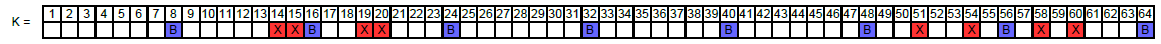
\includegraphics[scale=0.4]{images/K_complet.png}\end{center}
    \begin{center}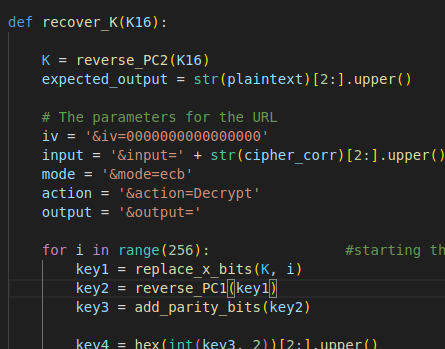
\includegraphics[scale=0.4]{images/boucle.png}\end{center}
     
	
\end{itemize}

\subsection{Question 2}

En appliquant la méthode décrite précédemment, on obtient la valeur de clé secréte suivante :

\color{red}
$K_{64} = 49$ $F4$ $64$ $F7$ $1C$ $9E$ $3E$ $E3$
\color{black}
\begin{figure}[h]
    \centering
    \begin{minipage}{0.4\textwidth}
        \centering
        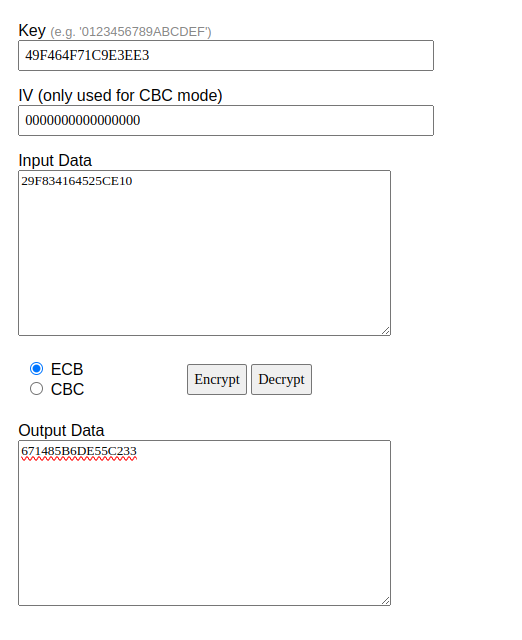
\includegraphics[width=\linewidth]{images/resultat_final.png}
        \caption{Résultat Obtenue}
        \label{fig:resultat1}
    \end{minipage}
    \hfill
    \begin{minipage}{0.4\textwidth}
        \centering
        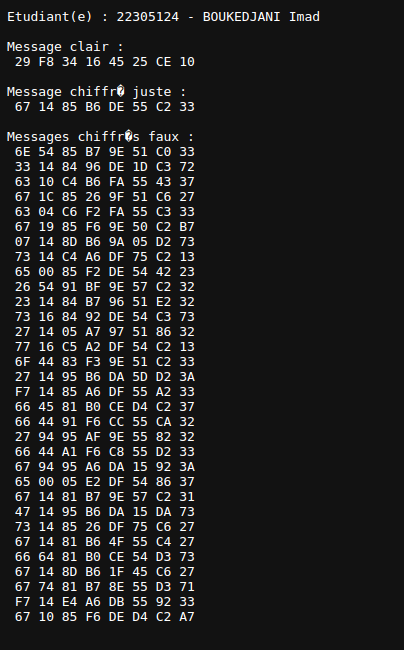
\includegraphics[width=\linewidth]{images/resultat_final2.png}
        \caption{Résultat Demandé}
        \label{fig:resultat2}
    \end{minipage}
\end{figure}
\newline

\section{Fautes sur les tours précédents}

\subsection{Faute provoquée sur la valeur de sortie $R_{14}$ du $14^{e}$ tour}

On sait que : 

\begin{itemize}
	\item $R_{15}=L_{14} \oplus f(K_{15}, R_{14})$ et $L_{15}=R_{14}$
	\item $R_{15*}=L_{14}* \oplus f(K_{15}, R_{14}*)$ et $L_{15*}=R_{14}*$
\end{itemize}

On obtient donc les équations suivantes : \newline
$R_{15} \oplus R_{15}* = L_{14} \oplus f(K_{15}, R_{14}) \oplus L_{14} \oplus f(K_{15}, R_{14}*)= f(K_{15}, R_{14}) \oplus f(K_{15}, R_{14}*)$ \newline \newline
On décompose pour obtenir $(E)$ (\textbf{ $R_{15}$ et $R_{15*}$ et $R_{16}$ et $R_{16*}$ et $L_{16}$ et $R_{16*}$  sont connues}): \newline \newline
$P^{-1}(R_{15} \oplus R_{15}* )=S_{i}(E(\ R_{14} )\oplus \ K_{15} )\oplus S_{i}(E(\ R_{14}* )\oplus \ K_{15} )$ \newline \newline
Or, $R_{14}=L_{15}=R_{16} \oplus f(K_{16}, L_{16})$ donne $P^{-1}(\ L_{15}  \oplus  R_{16} )_{b_{x}\to b_{y}}=S_i(E( L_{16}) \oplus \ K_{16}\color{black})_{b_{x}\to b_{y}}$ et \newline
$R_{14}*=L_{15}*=R_{16}* \oplus f(K_{16}, L_{16}*)$ donne $P^{-1}(\ L_{15}*\color{black} \oplus  R_{16}*\color{black})_{b_{x}\to b_{y}}=S_i(E( L_{16}*\color{black}) \oplus \ K_{16}\color{black})_{b_{x}\to b_{y}}$. \newline 
On fait donc une attaque exhaustive et on déduit les valeurs possibles pour $L_{15}$ et les $L_{15}*$. Cette attaque a donc une complexité de $O(2^{14})$. \newline \newline
Ensuite, pour chaque $L_{15}$ et $L_{15}*$ possible, on fait une attaque de complexité de $O(2^{14})$ pour trouver $K_{15}$ avec l'équation $(E)$. \newline
On a donc une complexité de $O(2^{14} \times 2^{14})=O(2^{28})$ sur l'attaque par faute provoquée sur la valeur de sortie $R_{14}$ du $14^{e}$ tour. Cette attaque reste \textbf{réaliste} car sa complexité est inférieure à $O(2^{80})$.

\subsection{Faute provoquée sur la valeur de sortie $R_{i}$ du $i^{e}$ tour}

Notons $O(2^a)$ la complexité de l'attaque DFA sur DES sur la valeur de sortie de $R_{15}$. Avec le paragraphe précédent, nous avons élaboré une attaque qui fonctionne sur n'importe quelle valeur de sortie de $R_i$ en multipliant la complexité de l'attaque du tour précédent par $O(2^a)$. On obtient donc les résultats suivants : 

\begin{itemize}
	\item Pour l'attaque sur le $15^e$ tour, la complexité est de $2^{14}$, qui est une attaque textbf{réaliste}. 
	\item Pour l'attaque sur le $14^e$ tour, la complexité est de $2^{28}$, qui est une attaque textbf{réaliste}. 
	\item Pour l'attaque sur le $13^e$ tour, la complexité est de $2^{42}$, qui est une attaque textbf{réaliste}. 
	\item Pour l'attaque sur le $12^e$ tour, la complexité est de $2^{56}$, qui est une attaque textbf{réaliste}. 
	\item Pour l'attaque sur le $11^e$ tour, la complexité est de $2^{70}$, qui est encore une attaque textbf{réaliste}. 
	\item Pour l'attaque sur le $10^e$ tour, la complexité est de $2^{84}$, qui est une attaque textbf{non réaliste} de nos jours puisqu'elle est \textbf{supérieure à $O(2^{80})$}. 
	
\end{itemize}

\section{Contre-mesures}

On distingue deux types de contre-mesures contre les attaques par injection de fautes. Les contre-mesures \textbf{algorithmiques} (qui utilisent les données calculées par la carte pour mettre en place un mécanisme de vérification) et les contre-mesures \textbf{physiques} (qui cherchent à protéger directement les composants de la carte d'une injection d'erreur).\newline
\begin{itemize}
	\item \textbf{Contre-mesures algorithmiques : } Comme expliqué précédemment, on cherche à mettre en place un mécanisme de vérification des calculs de la carte, cela en dégradant le moins possible le temps d’exécution de l’algorithme. La méthode la plus intuitive est de demander à la carte de calculer deux fois le même chiffrement et de comparer les chiffrés obtenus en sortie. Si ces chiffrés diffèrent, alors la carte refuse de renvoyer un quelconque résultat. Cette protection peut être valable car l’injection d’erreur est a priori aléatoire : il est assez peu probable que deux injections d’erreurs successives produisent la même erreur sur les mêmes bits. Ainsi, à quelques rares exceptions près, la carte ne renverra pas de chiffrés fautés : il n’est alors plus possible de mener l’attaque différentielle par injection de fautes. Le temps de calcul est alors deux fois celui du DES normal, ce qui reste acceptable étant donné qu’en pratique on utilise plutôt le triple DES (donc trois fois le temps d’un DES). \newline
	
	\item \textbf{Contre-mesures Physiques :} Une idée de protection physique serait d’ajouter des sondes pour surveiller les tensions et les températures dans les différents composants de la carte. Si certains seuils de tension ou de température sont dépassés, la carte considère qu’elle n’est plus en état de fonctionnement normal et cesse son activité jusqu’à ce que les seuils redeviennent acceptables. Avec ce type de protection, le temps de calcul reste inchangé. Cependant, cette méthode n’est pas toujours adaptée et nécessite une réflexion préalable : il est crucial de s'assurer que des éléments extérieurs naturels (comme une température plus élevée dans un pays chaud) ne provoquent pas le dépassement des seuils, ce qui arrêterait le fonctionnement de la carte.
\end{itemize}

\end{document}